\graphicspath{{Images/}}
\hypersetup{linkcolor=blue, urlcolor=blue}

\vspace{170pt}

\section{Nastavení prostředí}

\begin{spacing}{1.5}
    \fontsize{14}{14}\selectfont
    Tento projekt byl vykonan v \href{https://www.arduino.cc/en/software}{Arduino IDE}. pro spuštění projektu je potřeba nastavit prostředí. Na začatku je potřeba uvést správce ESP32. Pro to jdete do \textbf{File -> }\textbf{Preferences}
    
\begin{figure}[h]
    \centering
    \subfigure{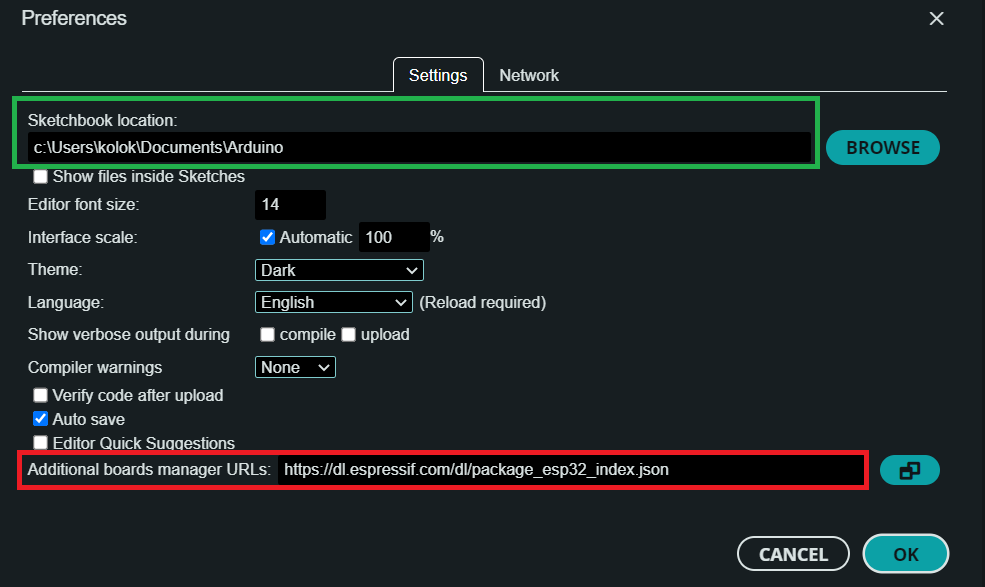
\includegraphics[scale=0.75]{img/preferences.png}}
    \caption{Je potřeba uvést \href{https://dl.espressif.com/dl/package_esp32_index.json}{spravce desky ESP32}}.
    \label{step}
\end{figure} 

\end{spacing}

\subsection{ESP32 Manager}

\begin{spacing}{1.5}
\fontsize{14}{14}\selectfont
Dále je potřeba nainstalovat spravce ESP32, který obsahuje knihovny. Pro to jdete do \textbf{Boards Manager} a nainstalujte esp32 od Espressif Systems.
\end{spacing}

\vspace{10pt}

\subsection{Připojení desky}
\begin{spacing}{1.5}
\fontsize{14}{14}\selectfont
Nyní můžeme přejit k připojení desky. Připojte desku přes micro-USB k počitači. Zvolte desku ESP32 Dev Module a port COM(USB).  
\end{spacing}
